\chapter[Implementación]{
  \label{chp:implementacion}
  IMPLEMENTACIÓN
}
\thispagestyle{numberingStyle}
\pagestyle{numberingStyle}



\section{Estructura de la aplicación}
\subsection{Estructura proyecto Java}
Para la implementación del modelo y la aplicación web, se ha elaborado un proyecto Maven con los siguientes módulos:
\\
\\

\begin{figure}[H]
\centering
\fbox{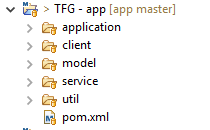
\includegraphics[
   keepaspectratio=true
]{./06_Implementacion/img/estructuraglobaljava.png}}
\caption{Estructura proyecto Java}
\end{figure}


\begin{itemize}
	\item \textbf{TFG - app: } Es el proyecto Maven de la aplicación Java. Está formado por diferentes módulos que forman la aplicación:
	\begin{itemize}
		\item \textbf{Application: }Es un módulo donde se encuentra la aplicación web y, que además, contiene un submódulo encargado de empaquetar como WAR la capa de servicios implementada en el módulo \textit{Service}.
		\item \textbf{Client: }Es el módulo correspondiente a la capa de acceso a servicios definida en el diseño de la aplicación. 
		\item \textbf{Model: } Módulo donde reside la persistencia y la lógica de negocio de la aplicación.
		\item \textbf{Service: }Es el módulo que define e implementa la capa de servicios.
		\item \textbf{Util: } Módulo de utilidad. Aporta clases y funciones comunes a los demás módulos.
		\item \textbf{pom.xml: }Archivo utilizado por Maven para la construcción del proyecto, manteniendo la gestión de las dependencias y el orden de construcción de los módulos.
	\end{itemize}
\end{itemize}

Con esta separación en módulos conseguimos hacer más independiente cada uno de los módulos que formarán el desplegable de la aplicación. De tal manera, que si queremos utilizar otra implementación de persistencia, simplemente tenemos que reemplazar el JAR generado por dicho módulo por el que queramos utilizar, en el archivo de aplicación web (WAR).

\subsubsection*{Módulo Model}
El módulo \textit{model} de la aplicación está compuesto por: \textit{core} y \textit{persistence}.

\begin{figure}[H]
\centering
\fbox{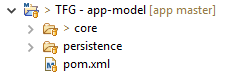
\includegraphics[
   keepaspectratio=true
]{./06_Implementacion/img/estructuramodeljava.png}}
\caption{Estructura módulo \textit{model}}
\end{figure}

En el submódulo \textit{persistence} se implementa toda la persistencia de datos, desde las clases persistentes hasta las definiciones e implementaciones de los DAOs. Por su parte, en el submódulo \textit{core} se define e implementa la lógica de negocio.

\subsubsection*{Estructura directorios Model - Persistence}
\begin{figure}[H]
\centering
\fbox{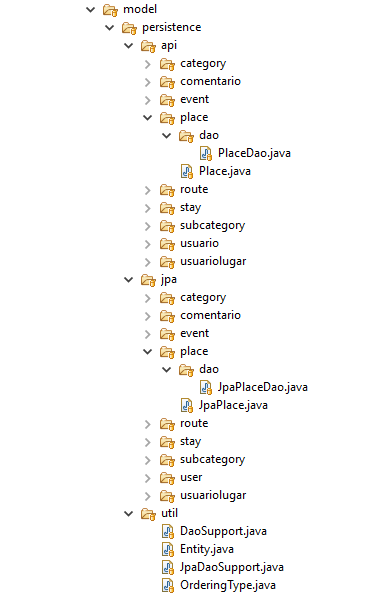
\includegraphics[
   keepaspectratio=true
]{./06_Implementacion/img/estructuramodelpersistence.png}}
\caption{Estructura módulo \textit{model-persistence}}
\end{figure}

\begin{itemize}
	\item \textbf{src/main/java/ ../model/persistence/api. }Es el directorio donde se encuentran todas las definiciones de las clases persistentes (Ej: Place.java) y los DAOs (Ej: PlaceDao.java).
	\item \textbf{src/main/java/ ../model/persistence/jpa. }Directorio donde residen las implementaciones de las definiciones anteriores (Ej: JpaPlace.java, JpaPlaceDao.java). Como su nombre indica, se hace uso del API de persistencia JPA. 
	\item \textbf{src/main/java/ ../model/persistence/util. }Es el directorio donde se incluyen clases de utilidad (Ej: DaoSupport y JpaDapSupport, para la implementación de los DAOs).
\end{itemize}

\subsubsection*{Estructura directorios Model - Core}
\begin{figure}[H]
\centering
\fbox{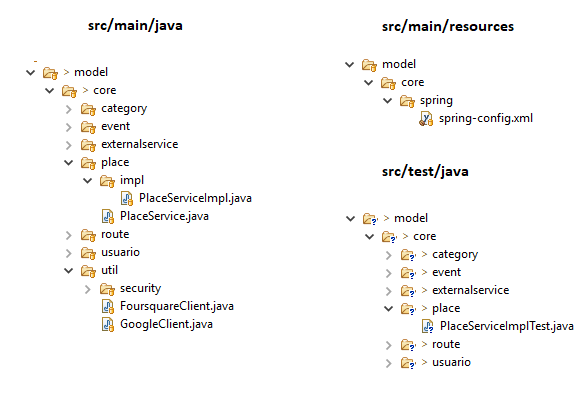
\includegraphics[
   keepaspectratio=true
]{./06_Implementacion/img/estructuramodelcore.png}}
\caption{Estructura módulo \textit{model-core}}
\end{figure}

\begin{itemize}
	\item \textbf{src/main/java/ ../model/core. }Directorio donde se especifica e implementa la lógica de negocio de la aplicación.
	\item \textbf{src/main/java/ ../model/core/util. }Directorio de utilidad que incluye los clientes de las APIs externas.
	\item \textbf{src/test/java/ ../model/core. }Incluye las pruebas automatizadas para cada uno de lo servicios de la lógica de negocio.
\end{itemize}


\newpage
\subsubsection*{Módulo Service}
El módulo \textit{service} de la aplicación está compuesto por los submódulos \textit{api} y \textit{core}.

\begin{figure}[H]
\centering
\fbox{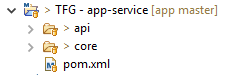
\includegraphics[
   keepaspectratio=true
]{./06_Implementacion/img/estructuraservice.png}}
\caption{Estructura módulo \textit{service}}
\end{figure}


\subsubsection*{Estructura directorios Service - Api}
\begin{figure}[H]
\centering
\fbox{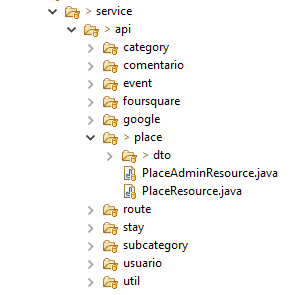
\includegraphics[
   keepaspectratio=true
]{./06_Implementacion/img/estructuraserviceapi.png}}
\caption{Estructura módulo \textit{service-api}}
\end{figure}

\begin{itemize}
	\item \textbf{src/main/java/ ../service/api. } Directorio donde se definen cada uno de los recursos web mediante la especificación de la API de JAX-RS. Esta API ofrece el soporte para la creación de servicios web, que ofrecerán remotamente, los servicios de la capa modelo. En la figura, se puede observar la definición de dos recursos web, como son: \textit{PlaceResource.java} y \textit{PlaceAdminResource.java}.
\end{itemize}


\subsubsection*{Estructura directorios Service - Core}
\begin{figure}[H]
\centering
\fbox{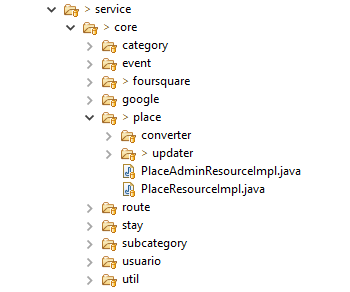
\includegraphics[
   keepaspectratio=true
]{./06_Implementacion/img/estructuraservicecore.png}}
\caption{Estructura módulo \textit{service-core}}
\end{figure}

\begin{itemize}
	\item \textbf{src/main/java/ ../service/core. } Directorio con las implementaciones para cada uno de los recursos definidos en el submódulo \textit{service-api}. Se pueden observar las clases \textit{PlaceResourceImpl.java} y \textit{PlaceAdminResourceImpl.java} que implementan las clases mostradas en el submódulo anterior.
	\begin{itemize}
		\item \textbf{../service/core/*/converter. }Directorio con las clases necesarias para la conversión de objetos persistentes a objetos de transferencia de datos, y viceversa.
		\item \textbf{../service/core/*/updater. }Directorio con las clases necesarias para la creación del objeto persistente a modificar a partir del objeto de transferencia de datos recibido. 
		\item \textbf{../service/core/util. }Directorio en el que se encuentran clases que ofrecen funcionalidades como la conversión de excepciones Java a respuestas HTTP, validadores de datos de entrada, etc...
	\end{itemize}
\end{itemize}



\subsubsection*{Módulo Application}
\begin{figure}[H]
\centering
\fbox{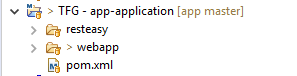
\includegraphics[
   keepaspectratio=true
]{./06_Implementacion/img/estructuraapplication.png}}
\caption{Estructura módulo \textit{application}}
\end{figure}

Formado por los submódulos \textit{resteasy} y \textit{webapp}. El primero de ellos será el encargado de obtener los servicios definidos e implementados en el módulo \textit{service} y ofrecerlos como servicios web. 

Por su parte, el módulo \textit{webapp} será el encargado de ofrecer una aplicación web, accesible mediante navegador web. 



\subsubsection*{Estructura directorios Application - Resteasy}
\begin{figure}[H]
\centering
\fbox{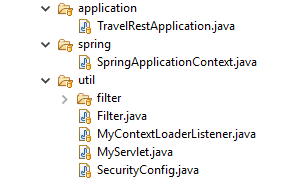
\includegraphics[
   keepaspectratio=true
]{./06_Implementacion/img/estructuraapplicationresteasy.png}}
\caption{Estructura módulo \textit{application-resteasy}}
\end{figure}

\begin{itemize}
	\item \textbf{src/main/java/ ../application/resteasy. }
	\begin{itemize}
		\item \textbf{../application/resteasy/application. }Directorio con la clase encargada de añadir al contenedor de la aplicación los objetos definidos en la capa de servicios.		
		\item \textbf{../application/resteasy/filter. }Directorio en el que se encuentran los filtros de la aplicación.
		\item \textbf{../application/resteasy/spring. }Directorio con la clase encargada de obtener los objetos del contenedor de Spring y poder incorporarlos al contenedor de la aplicación.
	\end{itemize}
\end{itemize}



\subsubsection*{Estructura directorios Application - Webapp}
\begin{figure}[H]
\centering
\fbox{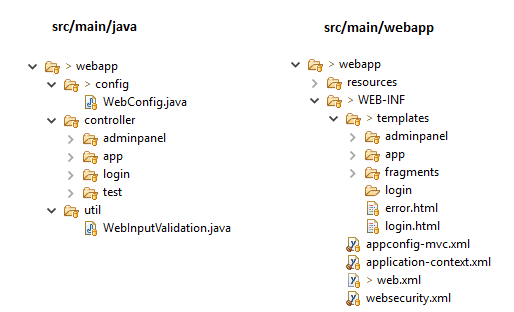
\includegraphics[
   keepaspectratio=true
]{./06_Implementacion/img/estructuraapplicationwebapp.png}}
\caption{Estructura módulo \textit{application-webapp}}
\end{figure}

\begin{itemize}
	\item \textbf{src/main/java. }
	\begin{itemize}
		\item \textbf{../application/webapp/config. }Directorio donde residen archivos de configuración de la aplicación.
		\item \textbf{../application/webapp/controller. }Directorio en el que se encuentran implementados los controladores de la aplicación.
		\item \textbf{../application/webapp/util. }Directorio con las clases de utilidad.
	\end{itemize}
	\item \textbf{src/main/webapp. }
	\begin{itemize}
		\item \textbf{../application/webapp/resources. }Directorio con los ficheros que aportan un mejor aspecto a la web. Incluye, archivos JavaScript, CSS e imágenes.
		\item \textbf{../application/webapp/WEB-INF. }Directorio en el que se encuentran las plantillas HTML utilizadas para crear las páginas web.
	\end{itemize}
\end{itemize}


\subsubsection*{Módulo Client}
\begin{figure}[H]
\centering
\fbox{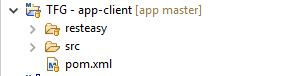
\includegraphics[
   keepaspectratio=true
]{./06_Implementacion/img/estructuraclient.png}}
\caption{Estructura módulo \textit{client}}
\end{figure}

El módulo \textit{client} está compuesto, únicamente, del módulo \textit{resteasy}. Este módulo, define e implementa un cliente para la aplicación REST anteriormente comentada.


\subsubsection*{Estructura directorios Client - Resteasy}
\begin{figure}[H]
\centering
\fbox{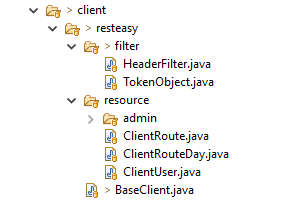
\includegraphics[
   keepaspectratio=true
]{./06_Implementacion/img/estructuraclientresteasy.png}}
\caption{Estructura módulo \textit{client-resteasy}}
\end{figure}

\begin{itemize}
	\item \textbf{src/main/java/ ../client/resteasy. }
	\begin{itemize}
		\item \textbf{../resteasy/filter. }Directorio donde residen los filtros utilizados por el cliente.
		\item \textbf{../resteasy/resource. }Directorio en el que se encuentran implementados los clientes específicos para cada servicio.
	\end{itemize}
\end{itemize}

\newpage
\subsection{Estructura proyecto Ionic}
Ionic presenta una estructura típica de proyecto Cordova donde se pueden instalar complementos nativos y crear archivos de proyecto, específicos para cada plataforma. La estructura de los archivos con el código fuente de la aplicación es la siguiente:

\begin{figure}[H]
\centering
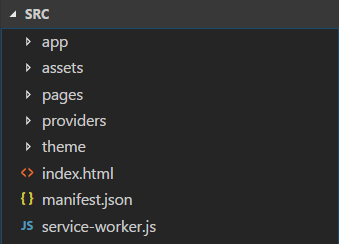
\includegraphics[
   keepaspectratio=true
]{./06_Implementacion/img/estructuraionicsrc.png}
\caption{Estructura aplicación \textit{Ionic}}
\end{figure}

\begin{itemize}
	\item \textbf{src/index.html. }Punto de entrada de la aplicación que tiene como propósito la configuración de \textit{scripts} y hojas de estilo para arrancar la aplicación.
	\item \textbf{src/app. }Directorio con las clases que inician la aplicación.
	\item \textbf{src/assets. }Directorio que almacena recursos de estáticos, como imágenes, iconos, etc...
	\item \textbf{src/pages. }Directorio en el que se encuentran las diferentes vistas y controladores que forman la aplicación.
	\item \textbf{src/providers. }Directorio que incluye las clases que implementan el acceso a los servicios y clases que implementan determinadas funcionalidades en la aplicación.
	\item \textbf{src/theme. }Directorio con las clases encargadas de especificar ciertos aspectos de estilo de la aplicación.
\end{itemize}


\subsubsection*{Estructura directorio pages}
En la siguiente figura, se muestra el subdirectorio \textit{pages}, que incluye todas las vistas y controladores de la aplicación.
\begin{figure}[H]
\centering

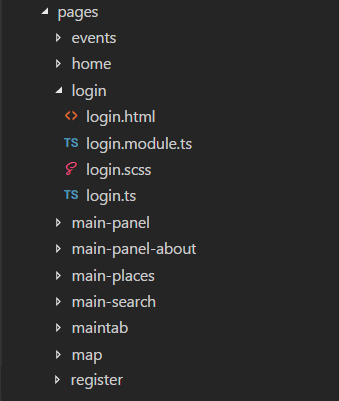
\includegraphics[
   keepaspectratio=true
]{./06_Implementacion/img/estructuraionicsrcpages.png}
\caption{Estructura aplicación \textit{Ionic - pages}}
\end{figure}

Para cada \textit{page} tenemos:
\begin{itemize}
	\item Un archivo HTML que contiene la vista de la página.
	\item Un archivo SCSS que contiene los estilos de la vista.
	\item Dos archivos TypeScript. Uno que actúa de controlador y otro que sirve para la configuración de las vistas.
\end{itemize}



\section{Implementación capa modelo}

\subsection{Persistencia}
Para la implementación de la persistencia de la aplicación se han seguido las definiciones especificadas en la API de persistencia para la plataforma Java, conocida comúnmente como JPA. Esta API nos proporciona una gestión de los datos relacionales en nuestra aplicación Java.


Puesto que JPA solo define un conjunto de interfaces, es necesaria una implementación de las mismas, que en este caso, será gracias al framework de Hibernate. Hibernate no solo implementa las especificaciones de JPA sino que también incorpora funcionalidades propias.


\subsubsection*{Implementación clases persistentes}
A continuación se mostrará un ejemplo de una entidad con las anotaciones definidas por JPA.

\begin{figure}[H]
\centering
\fbox{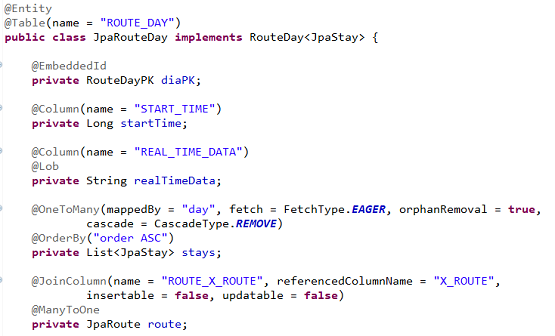
\includegraphics[
   keepaspectratio=true
]{./06_Implementacion/img/implclasespersist.png}}
\caption{Implementación clases persistentes}
\end{figure}

A continuación se explican, brevemente, las anotaciones JPA empleadas.

\begin{itemize}
	\item \textbf{@Entity. }Declara una clase POJO como entidad persistente. 
	\item \textbf{@Table. }Especifica la tabla empleada para la clase marcada como @Entity. 
	\item \textbf{@EmbeddedId. }Denota una clave primaria compuesta. Esta será una clase marcada por @Embeddable. Se aplica sobre un campo o propiedad persistente de la clase.
	\item \textbf{@Column. }Anotación utilizada para \textit{mapear} una columna con la propiedad o campo de la clase. El atributo \textit{name} permite especificar el nombre de la columna.
	\item \textbf{@Lob. }Determina que la propiedad debe persistir como una estructura que permita almacenar gran cantidad de información.
	\item \textbf{@OneToMany. }Define una relación de uno a muchos entre dos entidades. 
	\item \textbf{@OrderBy. }Especifica el orden de los elementos de la colección cuando son recuperados.
	\item \textbf{@JoinColumn. }Determina una columna para unir una entidad de asociación.
	\item \textbf{@ManyToOne. }Define una relación muchos a uno.
\end{itemize}



\subsubsection*{Implementación DAOs}
Como se ha comentado en el apartado de \textit{Diseño}, se ha elaborado un DAO genérico que implementa un conjunto de funcionalidades básicas. Para las consultas a la base de datos, realizadas por el DAO, se ha utilizado \textit{JPA Criteria API}, que nos permite definir estas consultas mediante la creación de una serie de objetos Java. A continuación, se muestra un ejemplo de uso de esta API.

\begin{figure}[H]
\centering
\fbox{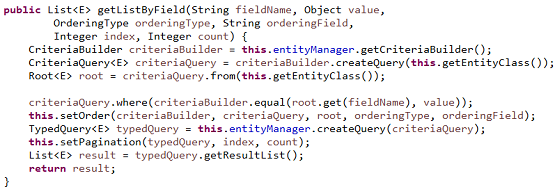
\includegraphics[
   keepaspectratio=true
]{./06_Implementacion/img/impldao.png}}
\caption{Implementación consultas DAO}
\end{figure}

En este ejemplo, se define el método \textit{getListByField(...)} que nos devolverá la lista de objetos que cumplan el filtro aplicado. Como se puede observar en la imagen, la consulta a la base de datos se ha realizado mediante la utilización de las clases ofrecidas por la API de Criteria, delegando en ellas la construcción de la \textit{query} necesaria.


\subsubsection*{Gestión de la transaccionalidad}
La lógica de negocio de la aplicación hace uso de los DAOs creados anteriormente y que realizan diferentes operaciones sobre la base de datos. Debido a que en un mismo caso de uso pueden realizar diferentes operaciones de los DAOs, es necesario crear una transacción que nos permita ejecutar todas esas acciones contra la base de datos en bloque y que, en caso de que alguna produjese un error, poder deshacer los cambios ocasionados por las demás. También son necesarias para operar sobre los mismos datos que estén manejados por dos o más hilos de ejecución.

Para ello, será necesario anotar estos métodos con la anotación \textit{@Transactional}. Con esta anotación, se empezará una transacción antes de la primera línea del método y se terminará justo después de la última, permitiendo ejecutar todo lo que esté dentro del método en una misma transacción.

\begin{figure}[H]
\centering
\fbox{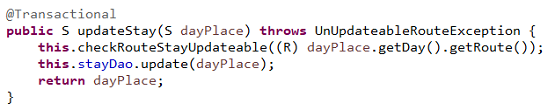
\includegraphics[
   keepaspectratio=true
]{./06_Implementacion/img/impltransactional.png}}
\caption{Implementación ejemplo transaccionalidad}
\end{figure}

En la figura 8.17, se define el método \textit{updateStay} marcado con la anotación comentada anteriormente, de forma que, todas las operaciones ejecutadas dentro del método se encontrarán dentro de una misma transacción. 


\section{Implementación capa servicios}
La aplicación está formada por una serie de servicios web REST que ofrecen las funcionalidades de la capa modelo remotamente. Como se había comentado, estos servicios han sido elaborados siguiendo las especificaciones establecidas por la API JAX-RS.

A continuación, se muestra un ejemplo de un recurso web, donde se explica, brevemente, la función de cada anotación.


\begin{figure}[H]
\centering
\fbox{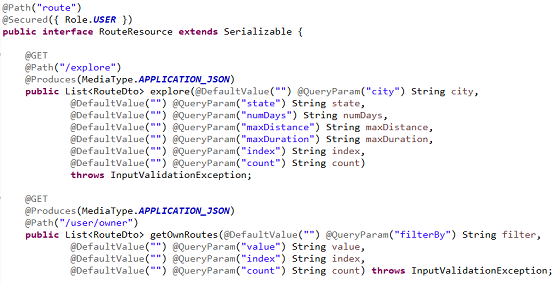
\includegraphics[
   keepaspectratio=true
]{./06_Implementacion/img/implapirest.png}}
\caption{Implementación ejemplo anotaciones JAX-RS}
\end{figure}

\begin{itemize}
	\item \textbf{@Path. }Identifica la URI en la que responderá un método o recurso de la clase. Toma un valor relativo, siendo la URI base el \textit{path} de la aplicación.
	\item \textbf{@Secured. }Anotación personalizada. Tiene el objetivo de marcar el recurso como seguro de manera que se aplique un filtro de autenticación en cada petición.
	\item \textbf{@GET. }Indica que el método anotado responde a solicitudes HTTP GET.
	\item \textbf{@Produces. }Define el \textit{mediatype} que pueden generar los métodos. Análogamente, existe la anotación @Consumes, que define el \textit{mediatype} que acepta el método.
	\item \textbf{@QueryParam. }Vincula el valor del parámetro HTTP a uno del método.
	\item \textbf{@DefaultValue. }Especifica un valor predeterminado para @QueryParam.
\end{itemize}


\section{Implementación autenticación y autorización}

\subsection{Implementación autenticación}

Se ha seguido un proceso de autenticación sin estado con el uso de \textit{Tokens}. Nuestro modelo ofrece una API REST \textit{stateless}, es decir, sin información de estado, donde los tokens son almacenados en lado del cliente, permitiendo que la aplicación sea totalmente escalable.

Para la implementación, se ha seguido el estándar JWT (JSON Web Token) que define una forma compacta y autónoma de transmitir de forma segura información entre dos partes mediante un objeto JSON.


\begin{figure}[H]
\centering
\fbox{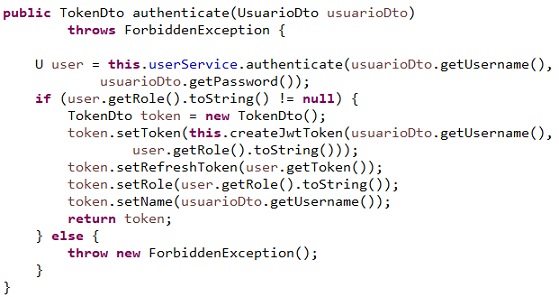
\includegraphics[
   keepaspectratio=true
]{./06_Implementacion/img/implautenticacion1.png}}
\caption{Implementación autenticación}
\end{figure}

En la figura anterior, se muestra la funcionalidad \textit{authenticate}. En este método, se delega al servicio \textit{userService} la comprobación de las credenciales ofrecidas por el usuario. Si la comprobación es correcta, se procede a la creación del token que es devuelto como respuesta al usuario.

\begin{figure}[H]
\centering
\fbox{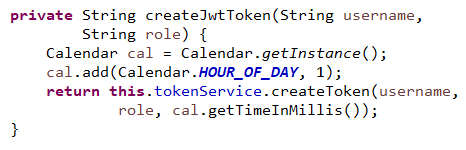
\includegraphics[
   keepaspectratio=true
]{./06_Implementacion/img/implautenticacion2.png}}
\caption{Implementación creación token}
\end{figure}

La creación del token se delega a la librería Java JWT, a través del servicio \textit{tokenService}, que es el encargado de elaborar las tres partes fundamentales de un JSON Web Token, que son: la cabecera, el \textit{payload} y la firma. El payload puede estar formado por diferentes atributos, en este caso, lo forman: el nombre de usuario, el rol del usuario y la fecha de expiración del token, fijada en una hora. 




\begin{figure}[H]
\centering
\fbox{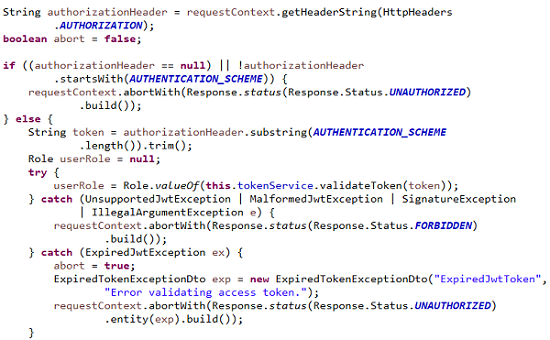
\includegraphics[
   keepaspectratio=true
]{./06_Implementacion/img/implautenticacion3.png}}
\caption{Implementación filtro autenticación}
\end{figure}

Por su parte, se elabora un filtro para la comprobación de la autenticación, comprobando que las peticiones incluyan la cabecera \textit{AUTHORIZATION} con el valor \textit{`Bearer + token'}. En el ejemplo anterior, de un trozo del filtro, podemos observar como se comprobará la existencia de dicha cabecera y se realizará la evaluación del token.

La evaluación del token se delegará al servicio \textit{tokenService} que obtendrá cada uno de los componentes que forman el token.


\subsection{Implementación autorización}
\subsubsection*{Implementación autorización por roles}
El sistema permitirá la realización de diferentes acciones en función del rol del usuario que solicite la acción. Para ello, en el filtro de autenticación, una vez validado el token, se obtiene del payload el rol especificado y se comprobará si este está incluido en la anotación \textit{@Secured}, comentada anteriormente, en el recurso web solicitado. Como se especificó, cada recurso web definido en la capa de servicios, incluye una anotación en la que se indica el rol necesario para realizar dichas operaciones.

\begin{figure}[H]
\centering
\fbox{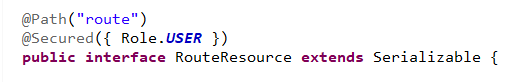
\includegraphics[
   keepaspectratio=true
]{./06_Implementacion/img/implautorizacion1.png}}
\caption{Implementación autorización recurso web - roles}
\end{figure}


En el filtro se extraerán los roles especificados en la cabecera \textit{@Secured} de cada recurso y se comprobarán con el rol incluido en el token. De tal manera, que se permitirá ejecutar la acción si ambos roles coinciden. Para el ejemplo anterior, sobre el recurso web \textit{route}, solo se permitirán acciones autenticadas por usuarios cuyo rol sea \textit{USER}.


\begin{figure}[H]
\centering
\fbox{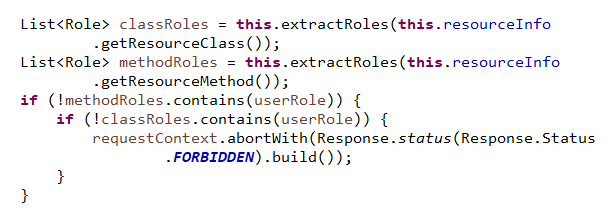
\includegraphics[
   keepaspectratio=true
]{./06_Implementacion/img/implautorizacion2.png}}
\caption{Implementación filtro autorización - roles}
\end{figure}

Con el filtro anterior conseguimos acciones autorizadas en función del rol especificado.


\subsubsection*{Implementación autorización basada en recursos}

Los roles son solo una parte de la autorización. Para evitar que un usuario acceda de forma no autorizada a un recurso creado por otro usuario, se utilizará el framework Spring Security. Con Spring Security se pueden definir expresiones en los métodos que permitan comprobar la autorización sobre cada recurso accedido.

\begin{figure}[H]
\centering
\fbox{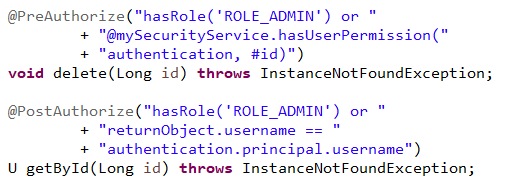
\includegraphics[
   keepaspectratio=true
]{./06_Implementacion/img/implautorizacion3.png}}
\caption{Implementación autorización servicios - basada en recursos}
\end{figure}

Para que estas anotaciones puedan ser utilizadas es necesario crear un objeto de autorización propio de Spring Security, donde se indica el nombre del usuario y el rol que tiene. Este objeto, se crea en el filtro de autenticación.

A continuación, se detallará cada una de las anotaciones y expresiones indicadas.

\begin{itemize}
	\item \textbf{@PreAuthorize. }Ejecuta la autorización antes de realizar el método. En la anotación se especifican los criterios de autorización.
	\begin{itemize}
		\item Que el usuario que realice la acción tenga el rol de \textit{ADMIN}.
		\item O que el usuario tenga los permisos necesarios. En este caso, se hace uso de una clase externa de utilidad, donde se comprobará que el recurso concreto al que se quiere acceder esté autorizado para el usuario que realiza la acción.
	\end{itemize}	 
		
	\item \textbf{@PostAuthorize. }Ejecuta la autorización después de realizar el método. Se especifican los siguientes criterios:
	\begin{itemize}
		\item Que el usuario que realice la acción tenga el rol de \textit{ADMIN}.
		\item O que el objeto de devuelto por el método pueda ser accedido por el usuario que realiza la acción.
	\end{itemize}
\end{itemize}


\newpage
\section{Implementación cliente web}

\subsection{Implementación acceso a servicios}

\begin{figure}[H]
\centering
\fbox{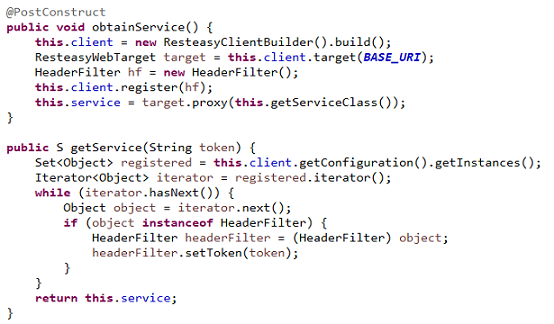
\includegraphics[
   keepaspectratio=true
]{./06_Implementacion/img/implclientweb.png}}
\caption{Implementación cliente web - Ejemplo acceso a servicios}
\end{figure}

La capa de acceso a los servicios implementada para el cliente web se elaborará mediante la implementación RESTEasy de la API JAX-RS Client. Con esta implementación se hace uso de \textit{proxy framework}, que actúa de manera opuesta a la especificación JAX-RS indicada en la capa de servicios. En vez de utilizar las anotaciones para determinar las peticiones entrantes al servicio REST, el cliente utiliza dichas anotaciones para construir la petición HTTP necesaria para enviar al servidor.

En el ejemplo, el método \textit{obtainService} se encargar de construir el cliente de RESTEasy. En él, se registra el filtro \textit{HeaderFilter}, utilizado para incluir el token de acceso en las peticiones. Una vez creado el cliente, se especifica a través del \textit{proxy}, la clase del servicio, que está anotada con la especificación de JAX-RS, para elaborar las peticiones HTTP necesarias.

El método \textit{getService} permite obtener el servicio indicando el token que se desea utilizar. Este método se encargará de indicar en el filtro, el token a incluir en la cabecera HTTP a la hora de elaborar la petición.


\subsection{Implementación controlador}
Para el cliente web se definen una serie de controladores encargados de recibir las peticiones del cliente final y ofrecer los datos. Estos controladores, han sido implementados mediante el framework Spring MVC. A continuación, se detalla el ejemplo de un controlador.

\begin{figure}[H]
\centering
\fbox{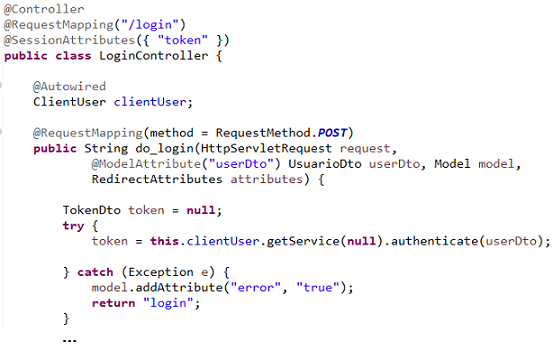
\includegraphics[
   keepaspectratio=true
]{./06_Implementacion/img/implcontrollerweb.png}}
\caption{Implementación cliente web - Ejemplo controlador}
\end{figure}

Este controlador se encarga de realizar las tareas de autenticación en el cliente web. Se pueden observar en la imagen, las anotaciones utilizadas para definir este controlador.

\begin{itemize}
	\item \textbf{@Controller. }Registra la clase como controlador.
	\item \textbf{@RequestMapping. }Anotación utilizada para asociar la clase o un método con una petición HTTP.
	\item \textbf{@SessionAttributes. }Define los atributos que deberán ser almacenados, transparentemente, en la sesión del navegador o en otro lugar de almacenamiento.
\end{itemize}

El método \textit{do\_login} recibe las peticiones POST con los datos del usuario a autenticar. El controlador hace uso del cliente creado en la capa de acceso a los servicios para realizar la petición al modelo. En función de la respuesta del modelo, el controlador se encargará de presentar una vista, u otra, al cliente.


\subsection{Implementación vistas}

\subsubsection*{Plantillas}

El desarrollo de las vistas en el servidor web ha sido elaborado mediante Thymeleaf, un motor de plantillas XML/XHTML/HTML5. Thymeleaf está completamente integrado con Spring MVC ofreciendo una sintaxis sencilla, permitiendo  la creación de plantillas de una manera elegante y con un código bien formateado.

\begin{figure}[H]
\centering
\fbox{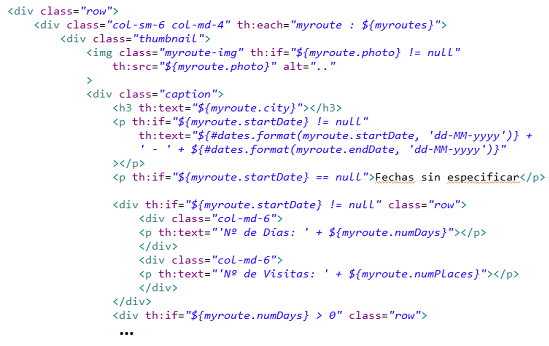
\includegraphics[
   keepaspectratio=true
]{./06_Implementacion/img/implvistaweb1.png}}
\caption{Implementación cliente web - Ejemplo vistas}
\end{figure}

En la figura anterior se muestra un ejemplo de una plantilla HTML creada con Thymeleaf. El controlador es el encargado obtener los datos y agregar los atributos necesarios a la vista a través de la clase \textit{Model} de Spring MVC. De esta manera, en la plantilla Thymeleaf podremos acceder a estos atributos mediante la sintaxis \textit{\$\{nombre\_del\_atributo\}}. Con expresiones como \textit{th:each}, para iterar una lista u objeto; \textit{th:if}, para comparar atributos o \textit{th:text}, para mostrar un atributo, podremos, fácilmente, manejar los atributos ofrecidos por el controlador en las vistas. 


\subsubsection*{AJAX}
El uso de la técnica de desarrollo AJAX nos permite mantener una comunicación asíncrona entre el cliente y el servidor web. Gracias a esta característica, podremos hacer que el cliente realice cambios sobre las páginas sin necesidad de recargarlas, mejorando la interactividad en la aplicación.

Thymeleaf Fragments son unos bloques de plantillas HTML que podemos renderizar directamente mediante AJAX. A continuación se mostrará un ejemplo de un \textit{fragment}.

\begin{figure}[H]
\centering
\fbox{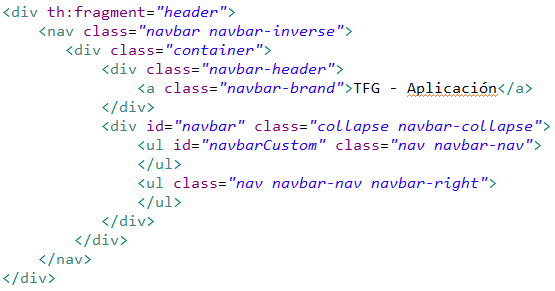
\includegraphics[
   keepaspectratio=true
]{./06_Implementacion/img/implvistaweb2.png}}
\caption{Implementación cliente web - Ejemplo fragments}
\end{figure}

En esta figura se muestra la definición de un fragment. En este caso se define un bloque HTML que incluye un diseño de una cabecera. Este fragment puede ser incrustado en otra plantilla Thymeleaf o ser cargado mediante AJAX. A continuación, se mostrará una figura en la que se podrá ver como se carga un fragment en una plantilla HTML mediante una petición AJAX.

\begin{figure}[H]
\centering
\fbox{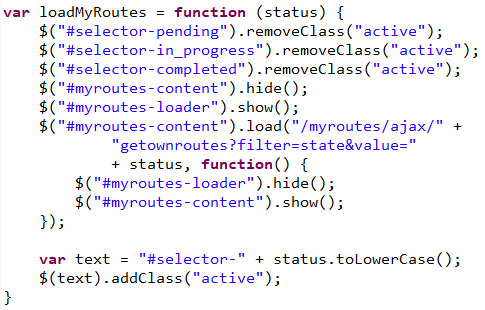
\includegraphics[
   keepaspectratio=true
]{./06_Implementacion/img/implvistaweb3.png}}
\caption{Implementación cliente web - Ejemplo AJAX}
\end{figure}

En este ejemplo, se define una función \textit{loadMyRoutes}. Cada vez que esta función sea ejecutada, mediante el método AJAX: \textit{load}, de jQuery, se realizará una petición al servidor consultando las rutas propias de un usuario. El controlador será el encargado de recibir esa petición y devolverá, cuando obtenga los datos, un fragment con los datos de las rutas que serán incorporados en el elemento \textit{\#myroutes-content}.


\section{Implementación cliente móvil}
El cliente móvil ha sido desarrollado con el SDK Ionic, construido sobre Angular y utilizando tecnologías web, como HTML o CSS.


\subsection{Implementación acceso a servicios}

\begin{figure}[H]
\centering
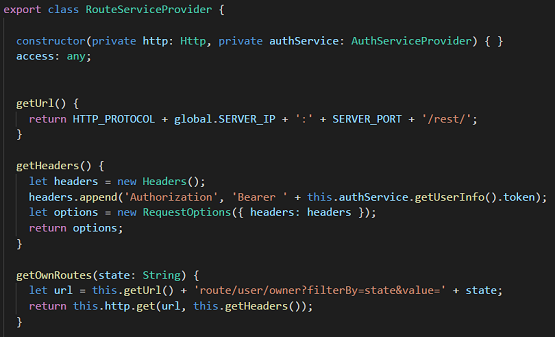
\includegraphics[
   keepaspectratio=true
]{./06_Implementacion/img/implclientmov.png}
\caption{Implementación cliente móvil - Ejemplo acceso a servicios}
\end{figure}

Las clases encargadas de acceder a los servicios del modelo hacen uso del módulo \textit{http} original de Angular. En la figura anterior, se muestra como se construye la URL de destino y se ejecuta la petición HTTP necesaria. El método \textit{getHeaders} permite crear las cabeceras de la petición e incluir el token de acceso necesario para autenticar dicha petición.

\subsection{Implementación vistas y controladores}
Como ya se comentó anteriormente, el cliente móvil sigue un diseño Modelo-Vista-VistaModelo (MVVM). En este caso se utilizará la palabra `Controlador' para referirnos al elemento VistaModelo. 

Los controladores inyectan un objeto \textit{\$scope} en las vistas. Las propiedades de este objeto estarán disponibles en la vista permitiendo que esta se actualice automáticamente a medida que se modifican los valores del objeto \textit{\$scope}. De esta forma se produce un enlace bidireccional de datos.

\begin{figure}[H]
\centering
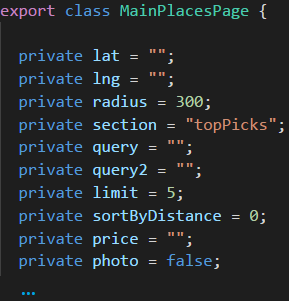
\includegraphics[
   keepaspectratio=true
]{./06_Implementacion/img/implcontrollermov.png}
\caption{Implementación cliente móvil - Ejemplo controlador}
\end{figure}


\begin{figure}[H]
\centering
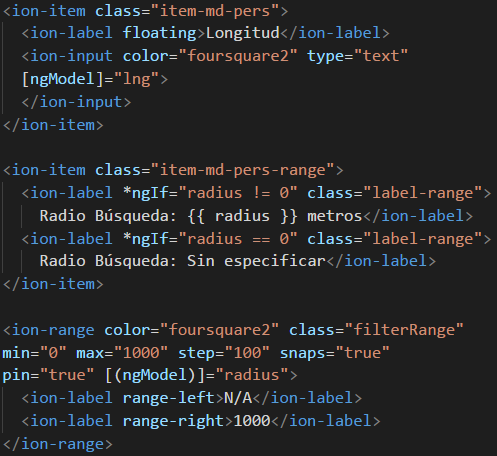
\includegraphics[
   keepaspectratio=true
]{./06_Implementacion/img/implcontrollermov2.png}
\caption{Implementación cliente móvil - Ejemplo vista}
\end{figure}


De las dos figuras mostradas, la primera hace referencia a la definición de un controlador. En él, se definen el conjunto de variables \textit{lat, lng, radius...} entre otras. Estas variables son inyectadas en la vista, como se puede observar en la figura 8.32. En la vista, se accede a estas variables del controlador mediante la directiva Angular \textit{ngModel}. 

Si se modifica el valor de estas variables en la vista, también se modificará en el controlador, permitiendo un intercambio dinámico de información entre los dos componentes.



\section{Compilación y despliegue}

En el CD adjunto se incluye un archivo \textit{README.txt} con las instrucciones necesarias para construir y desplegar la aplicación.














